\chapter{Hopcroft's Algorithm for Minimization of DFA} \label{chp:hopcroft}
Tree compression schemes that effectively exploit repetitive structures require efficient techniques for identifying and representing such repetitions in a compact manner. In our approach, we leverage deterministic finite automata (DFA) minimization as a foundational tool for recognizing and compressing recurring patterns within trees. Among the various DFA minimization algorithms, Hopcroft's algorithm stands out due to its optimal time complexity and efficiency in reducing state redundancies. This chapter provides the necessary theoretical background on Hopcroft's algorithm and DFA minimization, explaining their relevance to our proposed compression scheme. Also, we introduce a linear-time algorithm for minimizing acyclic deterministic finite automata, which is particularly suitable for identifying repetitive structures in trees. Let's start by introducing what are deterministic finite automata and why minimizing them is important for tree compression.

\section{Deterministic Finite Automata (DFA)}
\begin{definition}[Deterministic Finite Automaton] \label{def:dfa}
    A deterministic finite automaton (DFA) is a 5-tuple $M = (Q, \Sigma, \delta, q_0, F)$ where:
    \begin{itemize}
        \item $Q$ is a finite set of states
        \item $\Sigma$ is a finite set of input symbols (alphabet)
        \item $\delta: Q \times \Sigma \rightarrow Q$ is the transition function
        \item $q_0 \in Q$ is the initial state
        \item $F \subseteq Q$ is the set of final (accepting) states
    \end{itemize}
\end{definition}

The DFA processes an input string $s$ one symbol at a time by starting from the initial state $q_0$ and following transitions based on the input symbols. The string $s$ is accepted if the DFA ends in an accepting state after processing all input symbols, otherwise, it is rejected. The language recognized by a DFA is the set of all strings that lead to an accepting state. DFA are widely used in various applications, including lexical analysis, pattern matching, and formal language theory. 

\subsection{DFA Minimization}
The process of automata minimization consists in reducing the number of states in a DFA while preserving the language accepted by the DFA. The minimization of DFA is crucial for a variety of applications, such model checking, hardware design, and compilers, as it produces a more effective and compact representation of the automaton allowing for faster processing and reduced memory usage.

The minimization of DFA is a well-studied problem in automata theory, and there are several algorithms available for this purpose. One of the most popular algorithms for DFA minimization is the Hopcroft's algorithm, which was proposed by John Hopcroft in 1971 \cite{HOPCROFT1971189}. The Hopcroft's algorithm is an efficient and simple algorithm that can minimize a DFA in $O(n \log n)$ time, where $n$ is the number of states in the DFA.

\section{The Need for DFA Minimization in the novel scheme}
A key challenge in tree compression is the identification of structurally similar or identical subtrees. By modeling repetitive substructures as states in a DFA, we can transform the problem into one of minimizing redundant states, thereby reducing the size of the representation. DFA minimization ensures that equivalent substructures are merged efficiently, leading to a more compact encoding.

The minimized DFA provides a canonical representation of the repetitive structures, which can then be leveraged in our compression pipeline. This theoretical foundation enables us to systematically identify and encode tree patterns, ultimately improving the compression efficiency.

In the subsequent sections, we delve into the formal definition of the Hopcroft's algorithm. Then, we introduce an algorithm for minimizing acyclic DFAs in linear time, which is particularly relevant for identifying repetitive structures in trees. 

\section{Hopcroft's Minimization Algorithm}
Minimization of DFA is a classical and widely studied problem in automata theory and Formal Languages. It consists of finding the unique (up to isomorphism) finite automaton with the minimal number of states, recognizing the same regular language of a given DFA.

\begin{algorithm}
    \caption{Hopcroft's Algorithm for DFA Minimization} \label{alg:DFA_min}
    \begin{algorithmic}[1]
    \Require A DFA $M = (Q, \Sigma, \delta, q_0, F)$
    
    \State $P \gets \{F, Q \setminus F\}$ \Comment{Initial partition}
    \State $W \gets \{F\}$ \Comment{Working set initialized with final states}
    
    \While{$W \neq \emptyset$}
        \State Remove a set $A$ from $W$
        \ForAll{$c \in \Sigma$}
            \State $X \gets \{q \in Q \mid \delta(q, c) \in A\}$ \Comment{Predecessors of $A$ via $c$}
            \ForAll{$Y \in P$ such that $X \cap Y \neq \emptyset$ and $Y \setminus X \neq \emptyset$}
                \State Replace $Y$ in $P$ with $Y_1 = X \cap Y$ and $Y_2 = Y \setminus X$
                \If{$Y \in W$}
                    \State Replace $Y$ in $W$ with $Y_1$ and $Y_2$
                \Else
                    \State Add the smaller of $Y_1$ and $Y_2$ to $W$
                \EndIf
            \EndFor
        \EndFor
    \EndWhile
    
    \State \Return the minimized DFA built from partition $P$
    \end{algorithmic}
\end{algorithm}

Algorithm \ref{alg:DFA_min} works by iteratively refining a partition of the states until no further refinement is possible, meaning all states within each set of the partition are indistinguishable. The final partition represents the equivalence classes, which correspond to the states of the minimal DFA. Here's a step-by-step explanation based on the provided pseudocode:

\begin{enumerate}
    \item \textbf{Initialization:} The algorithm starts with an initial partition $P$ containing two sets: the set of final states $F$ and the set of non-final states $Q \setminus F$. These are the coarsest sets of potentially distinguishable states. A working set $W$ is initialized, typically containing the set of final states $F$ (or the smaller of the two initial sets as an optimization). $W$ holds the sets that are used as "splitters" to refine the partition $P$.

    \item \textbf{Refinement Loop:} The algorithm iterates as long as the working set $W$ is not empty. In each iteration, a set $A$ (a "splitter") is removed from $W$. Then, for each input symbol $c \in \Sigma$:
        \begin{itemize}
            \item Calculate the set $X = \{q \in Q \mid \delta(q, c) \in A\}$. This is the set of all states that transition *into* the set $A$ upon reading symbol $c$.
            \item For each set $Y$ currently in the partition $P$, check if $Y$ needs to be split by $X$. A split is necessary if some states in $Y$ are in $X$ and some are not (i.e., $X \cap Y \neq \emptyset$ and $Y \setminus X \neq \emptyset$). This indicates that states in $Y$ are distinguishable based on whether their $c$-transition leads into $A$.
            \item If $Y$ needs to be split, replace $Y$ in the partition $P$ with two new sets: $Y_1 = X \cap Y$ (states in $Y$ that transition into $A$) and $Y_2 = Y \setminus X$ (states in $Y$ that do not transition into $A$).
            \item Update the working set $W$: If the original set $Y$ was in $W$, remove $Y$ and add both new sets $Y_1$ and $Y_2$ to $W$. If $Y$ was not in $W$, add only the smaller of the two new sets ($Y_1$ or $Y_2$) to $W$. This optimization helps maintain the algorithm's efficiency.
        \end{itemize}

    \item \textbf{Termination:} The loop continues until the working set $W$ is empty. At this point, no set in the partition $P$ can be further refined. The partition $P$ now contains the final equivalence classes of states.

    \item \textbf{Result:} The final partition $P$ defines the states of the minimized DFA. Each set in $P$ corresponds to a single state in the minimal DFA, and transitions are defined based on the original DFA's transitions between these sets.
\end{enumerate}

The algorithm enables to compute equivalence classes of nodes in $O(n\log n)$, in particular, the Myhill-Nerode equivalence classes \cite{nerode1958linear, myhill1957finite}. The Myhill-Nerode theorem states that a language is regular if and only if it has a finite number of Myhill-Nerode equivalence classes. This theorem provides a powerful tool for determining the regularity of languages and is a cornerstone of automata theory. Let's formalize the concept of equivalence classes and the Myhill-Nerode theorem.

\begin{definition}[Equivalence Relation]
    For a language $L \subseteq \Sigma^*$ and any strings $x,y \in \Sigma^*$, we say $x$ is equivalent to $y$ with respect to $L$ (written as $x \approx_L y$) if and only if for all strings $z \in \Sigma^*$:
    \[ xz \in L \Leftrightarrow yz \in L \]
    That is, strings $x$ and $y$ are equivalent if they have the same behavior with respect to the language $L$ - either they both lead to acceptance or both lead to rejection when any suffix $z$ is appended.
\end{definition}

\begin{definition}[Regular Language]
    A language $L$ over an alphabet $\Sigma$ is called a \textbf{regular language} if it can be recognized by a deterministic finite automaton (DFA). Equivalently, a language is regular if it can be described by a regular expression or generated by a regular grammar. Regular languages form the simplest class in the Chomsky hierarchy of formal languages.
\end{definition}

\begin{theorem}[Myhill-Nerode theorem \cite{nerode1958linear,myhill1957finite}] \label{def:myhill-nerode}
    Let $L$ be a language over an alphabet $\Sigma$. Then $L$ is regular if and only if there exists a finite number of Myhill-Nerode equivalence classes for $L$. Specifically, the number of equivalence classes is equal to the number of states in the minimal DFA recognizing $L$.
\end{theorem}

\section{Minimization of acyclic DFA in linear time}
For our purpose, we will focus on a specific type of finite automaton: an acyclic deterministic finite automaton (or DAWG). An acyclic DFA is one where there are no cycles within the transitions. This property simplifies the minimization process since it ensures that every state can be reached from the start state through a unique path.

Let's start by giving the notion of directed acyclic word graph (DAWG):
\begin{definition}[DAWG]
    A \textbf{DAWG} (directed acyclic word graph) or automaton $\mathcal{A}$ is defined by the following 5-uple:
    \[
    \mathcal{A} = (Q, \Sigma, F, T, q_0),
    \]
    where
    \begin{itemize}
        \item $Q$ is a set of states;
        \item $\Sigma$ is an alphabet of finite cardinal denoted by $|\Sigma|$;
        \item $q_0$ is the initial state;
        \item $T$ is the subset of terminal states of $Q$;
        \item $F$ is a function of $Q \times \Sigma$ into $Q$ defining the transitions (arcs) of the automaton.
    \end{itemize}
\end{definition}

The state reached by a transition labeled $a$ from state $q$ is denoted by $q.a = F(q,a)$. This notation extends transitively to words: if $w$ is a word, then $q.w$ denotes the state reached by following the transitions labeled by each letter $w_1, w_2, \ldots, w_n$ of $w$. A word $w$ is accepted by the automaton if $q_0.w \in T$.

In this section, we will discuss an efficient algorithm for minimizing acyclic deterministic finite automata in linear time on the number of states \cite{revuz1992minimisation}. Let's start by giving some definitions and theorems introduced in the paper \cite{revuz1992minimisation}.

\begin{definition}[Height function]
    For a state $s$ in an automaton, the height $h(s)$ is defined as the length of the longest path starting at $s$ and going to a final state. 

    $$h(s) = \{|w||s.w \text{ is final}\}$$
\end{definition}

This height function induces a partition $\Pi_i$ of $Q$, where $\Pi_i$ denotes the set of states of height $i$.

\begin{definition}[Distinguished set]
    We say that a set $\Pi_i$ is distinguished if no pair of states in $\Pi_i$ are equivalent.
\end{definition}

\subsection{The algorithm}
The minimization algorithm introduced in \cite{revuz1992minimisation} operates by labeling each state with a unique identifier that represents the structure of the automaton from that state onward. It proceeds in the following steps:

\begin{enumerate}
    \item \textbf{Height Computation:} The height of each state is determined, where the height of a state is the length of the longest path from that state to a final state.
    \item \textbf{State Labeling:} Each state is labeled based on the structure of its transitions. The label consists of:
    \begin{itemize}
        \item Whether the state is final or not.
        \item The transitions, recorded as ordered pairs of symbols and target state identifiers.
    \end{itemize}
    \item \textbf{Lexicographic Sorting:} States at each height level are sorted lexicographically based on their labels using a bucket sort technique.
    \item \textbf{Merging Equivalent States:} After sorting, states with identical labels are merged, ensuring that equivalent states are unified.
\end{enumerate}

In details, the algorithm minimizes an acyclic deterministic finite automaton by leveraging the concept of state height. The algorithm partitions the states based on their height. It then processes these partitions in increasing order of height, starting from height 0.

The core idea relies on the `height property': If every $\Pi_j$ with $j < i$ is distinguished, then two states $p$ and $q$ in $\Pi_i$ (the set of states with height $i$) are equivalent if and only if for every letter $a$ in the alphabet $\Sigma$, the transitions $p.a$ and $q.a$ lead to the same state (or both are undefined).

The algorithm iteratively ensures that each $\Pi_i$ is distinguished. It starts with $\Pi_0$, where all states are trivially equivalent (as they are final states with no outgoing paths to other final states contributing to height) and merges them. Then, for each subsequent height $i$, it sorts the states in $\Pi_i$ based on their transitions. Specifically, states are grouped based on the target states of their transitions for each symbol in the alphabet. Since all lower levels ($j < i$) are already distinguished by the inductive step, states in $\Pi_i$ that have identical transitions for all symbols (leading to equivalent states in lower levels) are themselves equivalent according to the height property. These equivalent states are then merged.

This process uses a specialized lexicographic sorting technique (related to bucket sort) optimized for this task, which helps achieve linear time complexity relative to the size of the automaton (number of states and transitions). The algorithm leverages a technique similar to the one presented in \cite{aho1974design} for testing tree isomorphism. Specifically, Revuz adopt a renumbering scheme during the lexicographic sorting phase to optimize both time and space complexity. 

\subsection{Renumbering Scheme Explained}
The core minimization algorithm relies on sorting states at the same height level based on their transitions. A state $s$ can be represented by a label or tuple: $(F/NF, l_1, nl_1, l_2, nl_2, \dots, l_k, nl_k)$, where $F/NF$ denotes final/non-final status, $l_i$ is the $i$-th transition symbol (alphabet character), and $nl_i$ is the target state of that transition.

The challenge arises when performing the lexicographic sort (using repeated bucket sorts) on these labels, specifically concerning the $nl_i$ components. If the actual state numbers (ranging from $1$ to $|Q|$, the total number of states) are used directly as the values for $nl_i$:
\begin{itemize}
    \item The range of values for these components becomes large ($1$ to $|Q|$). This forces the bucket sort step that handles these components to use a bucket array of size $|Q|$, potentially making the sort non-linear in the size of the automaton if $|Q|$ is large compared to the number of transitions $e$.
    \item Alternatively, representing state numbers as strings of digits would increase the length of the labels by a factor proportional to $\log |Q|$, again potentially breaking the overall linear time complexity.
\end{itemize}

The renumbering scheme overcomes this issue by assigning temporary, small integer names to the target states ($nl_i$) during the sorting process for each height level $\Pi_i$. The key idea is that when sorting states at height $i$, we only need to distinguish between the equivalence classes of the target states $nl_i$ from lower levels ($j < i$), as those levels have already been processed and minimized. The renumbering scheme ensures that the bucket array size is bounded by the maximum of $|C|$ (the alphabet size) and $E_i$ (the total number of edges from states at height i). The renumbering function adopted is the following:

\begin{algorithm}
    \caption{Renumbering Function}
    \begin{algorithmic}[1]
        \Function{Renumber}{s, h, n}
            \If{$s.\text{ch} \ne h$}
                \State $s.\text{ch} = h$
                \State $s.\text{num} = n$
                \State $n = n + 1$
            \EndIf
            \State \Return $s.\text{num}$
        \EndFunction
    \end{algorithmic}
\end{algorithm}

\subsection{Pseudocode}
The paper presents the core minimization logic and a more detailed sorting (or distinguishing) algorithm separately. Here's a combined representation based on the `Final algorithm' section of the paper.

\begin{algorithm}
    \caption{Minimization Algorithm for Acyclic DFAs}  
    \begin{algorithmic}[1]
    \State Calculate height $h(s)$ for every state $s$.
    \State Create partitions $\Pi_i = \{s \in Q \mid h(s) = i\}$.
    \State Merge all states in $\Pi_0$.
    \For{$i := 1$ to $h(q_0)$} \Comment{$q_0$ is the initial state}
        \State \Comment{Distinguish states in $\Pi_i$ using the sorting/distinguishing algorithm below}
        \State Put states in $\Pi_i$ into a list $L$. \Comment{May pre-split by Final/NonFinal}
        \State Call Distinguish($L$)
        \State Merge resulting groups of equivalent states identified by Distinguish.
    \EndFor
    \end{algorithmic}
\end{algorithm}

Algorithm \ref{alg:distinguish} distinguishes states within a given height level $\Pi_i$. It iteratively refines partitions based on transitions. Each state $s$ is labeled with the following:
$$label(s) = (F/NF, l_1, nl_1, l_2, nl_2, \dots, l_k, nl_k)$$
where $F/NF$ indicates final/non-final, $l_k$ is the $k$-th transition symbol, and $nl_k$ is the (renumbered) target state name. The sorting happens component by component.

\begin{algorithm}[h]
    \caption{Distinguish Algorithm} \label{alg:distinguish}
    \begin{algorithmic}[1] 
        \Function{Distinguish}{List\_of\_States}
        \State Place List\_of\_States into QUEUE2 \Comment{Queue of lists of potentially equivalent states}
        \State $k := 0$ \Comment{Represents the component index of the label being compared}
        \Repeat
            \State Move QUEUE2 to QUEUE1; Clear QUEUE2
            \State $k := k + 1$
            \While{QUEUE1 not empty}
                \State Let $L$ be the first list in QUEUE1
                \State Clear Buckets $Q[1 \dots m]$ \Comment{$m$ depends on alphabet size and renumbered state names}
                \State Clear NONEMPTY list of bucket indices
                \While{$L$ not empty}
                    \State Let $S$ be the first state in $L$
                    \State Determine the $k$-th component value $v$ for state $S$
                    \If{$Q[v]$ is empty}
                        \State Add $v$ to NONEMPTY
                    \EndIf
                    \State Move $S$ from $L$ to bucket $Q[v]$
                \EndWhile
                \For{each index $v$ in NONEMPTY}
                    \If{Bucket $Q[v]$ contains more than one state}
                        \State Add $Q[v]$ as a list to QUEUE2 \Comment{These still need further distinguishing}
                    \ElsIf{$k$ corresponds to the end-of-label marker '$S$'}
                        \State Merge all states in $Q[v]$ (they are equivalent)
                    \EndIf
                \EndFor
            \EndWhile
        \Until{QUEUE2 is empty} \Comment{No more lists need refinement}
        \EndFunction
    \end{algorithmic}
\end{algorithm}

\textit{Note:} The pseudocode in the paper is slightly intertwined with the bucket sort details. This representation attempts to capture the logic described. The renumbering function is called implicitly when accessing $nl_j$. The handling of merging might occur after the Distinguish procedure completes for level $i$, or potentially within it as groups become fully distinguished. The pseudocode merges states within bucket Q[\$], which relates to the end-of-string marker in the generic sort; for state labels, equivalence is confirmed when a group remains together after checking all label components.

\subsection{Example}
Now we are going to see an example of reduction for a given DAWG. The DAWG is represented in figure \ref{fig:example_dawg} and, as we can notice, it is also a valid ordered rooted tree with $n = 11$ nodes, $e = 10$ edges and the following alphabet: $\Sigma = \{0, 1\}$. The node $a$ is the root of the tree and the initial state of the automaton, while the leaf nodes $e,g,h,i,l,m$ are final states.

\begin{figure}[H]
    \centering
    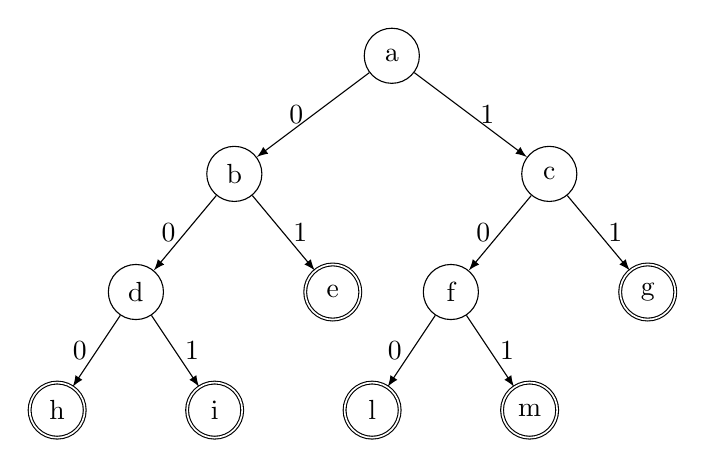
\begin{tikzpicture}[
        level distance=1.5cm,
        sibling distance=3cm,
        state/.style={circle, draw, minimum size=7mm},
        accepting/.style={circle, draw, double, minimum size=7mm},
        edge from parent/.style={draw, -latex},
        level 1/.style={sibling distance=4cm},
        level 2/.style={sibling distance=2.5cm},
        level 3/.style={sibling distance=2cm}
        ]
    
    \node[state] (a) {a}
        child {node[state] (b) {b} 
        child {node[state] (d) {d}
            child {node[accepting] (h) {h}}
            child {node[accepting] (i) {i}}
        }
        child {node[accepting] (e) {e}}
        }
        child {node[state] (c) {c}
        child {node[state] (f) {f}
            child {node[accepting] (l) {l}}
            child {node[accepting] (m) {m}}
        }
        child {node[accepting] (g) {g}}
        };
    
    % Etichette degli archi
    \path (a) -- (b) node[midway, left] {0};
    \path (a) -- (c) node[midway, right] {1};
    \path (b) -- (d) node[midway, left] {0};
    \path (b) -- (e) node[midway, right] {1};
    \path (c) -- (f) node[midway, left] {0};
    \path (c) -- (g) node[midway, right] {1};
    \path (d) -- (h) node[midway, left] {0};
    \path (d) -- (i) node[midway, right] {1};
    \path (f) -- (l) node[midway, left] {0};
    \path (f) -- (m) node[midway, right] {1};
    \end{tikzpicture}
    \caption{Example DAWG to be minimized}
    \label{fig:example_dawg}
\end{figure}

Now by applying the algorithm, we obtain minimized DAWG represented in figure \ref{fig:example_minimized_dawg}. Each node of the original DAWG is represented by a node in the minimized DAWG (equivalence classes). The edges represent transitions between these nodes. The root node $A$ is the initial state of the minimized DAWG, while the node $D$ is the final state.
\begin{figure}[H]
    \centering
    \begin{tikzpicture}[->, >=stealth, node distance=3cm, on grid, auto]
        \node[state, initial] (A) {A};
        \node[state] (B) [right=of A] {B};
        \node[state] (C) [right=of B] {C};
        \node[state, accepting] (D) [right=of C] {D};
    
        \path (A) edge [bend left] node {0} (B)
                edge [bend right] node[below] {1} (B)
            (B) edge [bend left] node {0} (C)
                edge [bend right] node[below] {1} (D)
            (C) edge [bend left] node {0} (D)
                edge [bend right] node[below] {1} (D);
    \end{tikzpicture}
    \caption{Minimized DAWG}
    \label{fig:example_minimized_dawg}
\end{figure}      

The equivalence classes of the nodes are listed in table \ref{tab:equivalence_classes}.
\begin{center}
    \begin{tabular}{|c|l|}
    \hline
    \textbf{Class} & \textbf{States} \\
    \hline
    A & $a$ \\
    B & $b, c$ \\
    C & $d, f$ \\
    D & $e, g, h, i, l, m$ \\
    \hline
    \end{tabular}
    \captionof{table}{Equivalence classes of the nodes}
    \label{tab:equivalence_classes}
\end{center}